\documentclass[a4paper,12pt]{article}

\usepackage{mystyle}
\usepackage{gensymb}

\graphicspath{ {images/} }


% https://tex.stackexchange.com/questions/5461/is-it-possible-to-change-the-size-of-an-arrowhead-in-tikz-pgf
\usetikzlibrary{arrows.meta}

% https://tex.stackexchange.com/questions/261591/arrow-above-text-like-widehat
\usepackage{esvect}

% https://tex.stackexchange.com/questions/32501/how-to-get-a-good-divisible-by-symbol
\DeclareRobustCommand{\divby}{%
  \mathrel{\vbox{\baselineskip.65ex\lineskiplimit0pt\hbox{.}\hbox{.}\hbox{.}}}%
}


\definecolor{light-cyan}{RGB}{0, 204, 204}
\definecolor{light-purple}{RGB}{138, 43, 226}


\author{Алексеев Василий}
\title{Семинар 3}
\date{15 + 21 сентября 2020}


\begin{document}
  \maketitle
  
  \tableofcontents

  \thispagestyle{empty}
  
  \newpage
  
  \pagenumbering{arabic}


  \section{Замена базиса и системы координат}
  
  Будем обозначать векторы базиса в виде строки:
  \[
    \bds e \hm= (\bds e_1, \bds e_2, \bds e_3)
  \]
  для случая базиса в $\RR^3$.
  Аналогично и для базисов в $\RR^2$, $\RR$.
  
  При заданном базисе $\bds e$ любой вектор пространства $\bds x$ однозначно определяется его компонентами в базисе:
  \[
    \bds x = x_1 \cdot \bds e_1 + x_2 \cdot \bds e_2 + x_3 \cdot \bds e_3
      \Rightarrow \bds x \leftrightarrow (x_1, x_2, x_3)^T
  \]
  поэтому, говоря о векторе, часто имеют в виду его компоненты в базисе (то понятия вектора как направленного отрезка и вектора как столбца из чисел взаимозаменяемы).
  Но это при фиксированном базисе.
  
  В пространстве существует больше одного базиса: любая тройка некомпланарных векторов в $\RR^3$ образует базис.
  Встаёт вопрос о том, как связаны компоненты одного и того же вектора в разных базисах\footnote{В приложениях бывает нужно переводить координаты радиусов-векторов точек из одной системы координат в другую.}
  
  \begin{figure}[h]
    \centering
    
    \includegraphics[width=0.5\columnwidth]{two-basises}
    
    \caption{Два разных базиса в пространстве.}
    \label{fig:two-basises}
  \end{figure}
  
  Пусть есть два базиса: $\bds e$ и $\bds e'$ (\ref{fig:two-basises}).
  Тогда векторы любого базиса можно разложить по системе векторов другого базиса.
  Разложим, например, векторы $\bds e$ по $\bds e'$:
  \begin{equation}\label{eq:e1-to-e2-via-system-of-equations}
    \left\{
      \begin{aligned}
        &\bds e_1 = a_{11} \cdot \bds e'_1 + a_{12} \cdot \bds e'_2 + a_{13} \cdot \bds e'_3\\
        &\bds e_2 = a_{21} \cdot \bds e'_1 + a_{22} \cdot \bds e'_2 + a_{23} \cdot \bds e'_3\\
        &\bds e_3 = a_{31} \cdot \bds e'_1 + a_{32} \cdot \bds e'_2 + a_{33} \cdot \bds e'_3
      \end{aligned}
    \right.
  \end{equation}
  
  Запись можно представить более компактно\footnote{Под результатом умножения строки из векторов $\bds e'$ на матрицу из чисел $S$ будем иметь в виду такую строку $\bds e$ из векторов, где каждый элемент равен линейной комбинации векторов умножаемой строки $\bds e'$ с коэффициентами, равными элементам соответственного столбца матрицы $S$. То есть по правилу умножения числовых матриц.}:
  \[
    \bds e = \bds e' S
  \]
  где $S$ называется \emph{матрицей перехода} от базиса $\bds e'$ к базису $\bds e$:
  \[
    S = \begin{pmatrix}
      a_{11} & a_{21} & a_{31}\\
      a_{12} & a_{22} & a_{32}\\
      a_{13} & a_{23} & a_{33}
    \end{pmatrix}
  \]
  во введённых ранее обозначениях (\ref{eq:e1-to-e2-via-system-of-equations}).
  
  Посмотрим теперь, как выражаются компоненты некоторого вектора $\bds x$ в одном базисе через его же компоненты, но в другом базисе.
  Имеем
  \begin{equation}\label{eq:same-vector-two-faces}
    \bds x = \bds e \bds x_e = \bds e' \bds x_{e'}
  \end{equation}
  где $\bds x$~---~вектор как направленный отрезок,
  $\bds x_e$~---~вектор-столбец, соответствующий $\bds x$ в базисе $\bds e$,
  $\bds x_{e'}$~---~вектор-столбец, соответствующий $\bds x'$ в базисе $\bds e'$.
  
  Теперь воспользуемся тем, что нам известно представление базиса $\bds e$ через вектора базиса $\bds e'$:
  \[
    \bds e \bds x_e = \bigl(\bds e' S\bigr) \bds x_e
      \stackrel{(\ref{eq:same-vector-two-faces})}{=} \bds e' \bds x_{e'}
  \]
  Так как умножение матриц ассоциативно, а также дистрибутивно относительно матричного сложения, мы можем перенести $\bds e' \bds x_{e'}$ влево и перегруппировать слагаемые:
  \[
    \bds e' \cdot \bigl(S \bds x_e - \bds x_{e'}\bigr) = \bds 0
  \]
  
  Из линейной независимости системы векторов $\bds e'$ получаем:
  \[
    S \bds x_e - \bds x_{e'} = \bds 0 \Leftrightarrow \bds x_{e'} = S \bds x_e
  \]
  
  Итак, в двух базисах компоненты векторов связаны так:
  \begin{equation}\label{eq:vector1-to-vector2}
    \boxed{
      \left\{
        \begin{aligned}
          &\bds e = \bds e' S\\
          &\bds x_{e'} = S \bds x_e
        \end{aligned}
      \right.
    }
  \end{equation}
  
  При этом, при переходе, наоборот, от базиса $\bds e$ к базису $\bds e'$
  можно написать аналогичное соотношение, но уже с другой матрицей перехода, которую обозначим за $S'$:
  \[
    \left\{
      \begin{aligned}
        &\bds e' = \bds e S'\\
        &\bds x_{e} = S' \bds x_{e'}
      \end{aligned}
    \right.
  \]

  \begin{figure}[h]
    \centering
    
    \includegraphics[width=0.5\columnwidth]{two-coords}
    
    \caption{Две системы координат в пространстве.}
    \label{fig:two-coords}
  \end{figure}

  Последний вопрос: как изменяются радиусы-векторы точек при смене системы координат (\ref{fig:two-coords})?
  Очевидно,
  \[
    \bds r_O(A) = \bds r_O(O') + \bds r_{O'}(A)
  \]
  где $\bds r_O(A)$~---~радиус-вектор точки $A$ в системе $O; \bds e$,
  $\bds r_{O'}(A)$~---~радиус-вектор точки $A$ в системе $O'; \bds e'$,
  и $\bds r_O(O')$~---~радиус-вектор, определяющий положение начала отсчёта $O'$ в системе $O; \bds e$.
  В системе $O'; \bds e'$ известно координатное представление вектора $ \bds r_{O'}(A)$.
  Для других же двух векторов $\bds r_O(A)$ и $\bds r_O(O')$ известны компоненты в базисе $O; \bds e$.
  Как записать соотношение выше через вектор-столбцы компонент векторов в базисах?
  Для этого надо все векторы представить в одном базисе.
  Из соотношения (\ref{eq:vector1-to-vector2}) мы можем выразить вектор $\bds r_{O'}(A)$ в базисе $\bds e$:
  \[
    \bds r_{O'}(A) = S' \bds x_{O'}(A)
  \]
  где $\bds x_{O'}(A)$~---~компоненты радиус-вектора точки $A$ в $O'; \bds e'$ и $S' \bds x_{O'}(A)$~---~компоненты \emph{того же} вектора в системе $O; \bds e$.
  Итого, получаем соотношение для компонент радиусов-векторов точки в разных системах координат:
  \begin{equation}\label{eq:point1-to-point2}
    \boxed{
      \left\{
        \begin{aligned}
          &\bds e' = \bds e S'\\
          &\bds x_O(A) = \bds x_O(O') + S' \bds x_{O'}(A)
        \end{aligned}
      \right.
    }
  \end{equation}
  то есть для нахождения координат точки в одной системе по её координатам в другой системе координат надо знать связь между векторами базисов и положение начала координат одной системы относительно другой.
  
  \begin{problem}[4.5]
    Есть две системы координат: $O; \bds e$ и $O'; \bds e'$.
    Координаты произвольной точки в первой системе обозначаются за $(x, y)$, координаты той же точки, но во второй системе координат~---~$(x', y')$.
    Известна связь между $(x, y)$ и $(x', y')$:
    \[
      \left\{
        \begin{aligned}
          &x = 2x' - y' + 5\\
          &y = 3x' + y' + 2
        \end{aligned}
      \right.
    \]
    
    Требуется найти
    \begin{itemize}
      \item Выражение $(x', y')$ через $(x, y)$.
      \item Координаты точки $O$ и компоненты векторов $\bds e_1, \bds e_2$ в системе $O'; \bds e'$.
      \item Координаты точки $O'$ и компоненты векторов $\bds e_1', \bds e_2'$ в системе $O; \bds e$.
    \end{itemize}
  \end{problem}
  
  \begin{solution}
    Перепишем связь между координатами точки в разных системах в матричном виде:
    \begin{equation}\label{eq:problem1-x-to-x-prime}
      \begin{pmatrix}
        x\\
        y
      \end{pmatrix}
      = \overbrace{\begin{pmatrix}
        2 & -1\\
        3 & 1
      \end{pmatrix}}^{S'}
      \begin{pmatrix}
        x'\\
        y'
      \end{pmatrix}
      + \begin{pmatrix}
        5\\
        2
      \end{pmatrix}
    \end{equation}
    
    Перепишем как
    \[
      \begin{pmatrix}
        2 & -1\\
        3 & 1
      \end{pmatrix}
      \begin{pmatrix}
        x'\\
        y'
      \end{pmatrix}
      = \begin{pmatrix}
        x - 5\\
        y - 2
      \end{pmatrix}
    \]
    
    И решим получившуюся систему относительно $(x', y')$ с помощью метода Крамера:
    \[
      \Delta = \begin{vmatrix} 2 & -1 \\ 3 & 1 \end{vmatrix} = 2 + 3 = 5 \not= 0
    \]
    \[
      \Delta_{x'} = \begin{vmatrix} x - 5 & -1 \\ y - 2 & 1 \end{vmatrix} = x + y - 7
    \]
    \[
      \Delta_{y'} = \begin{vmatrix} 2 & x - 5 \\ 3 & y - 2 \end{vmatrix} = -3x + 2y + 11
    \]
    
    И сами координаты:
    \[
      x' = \frac{\Delta_{x'}}{\Delta} = \frac{1}{5} x + \frac{1}{5} y - \frac{7}{5}\\
    \]
    \[
      y' = \frac{\Delta_{y'}}{\Delta} = -\frac{3}{5} x + \frac{2}{5} y + \frac{11}{5}
    \]
    
    Или в матричном виде:
    \begin{equation}\label{eq:problem1-x-prime-to-x}
      \begin{pmatrix}
        x'\\
        y'
      \end{pmatrix}
      = \overbrace{\begin{pmatrix}
        1/5 & 1/5\\
        -3/5 & 2/5
      \end{pmatrix}}^{S}
      \begin{pmatrix}
        x\\
        y
      \end{pmatrix}
      + \begin{pmatrix}
        -7/5\\
        11/5
      \end{pmatrix}
    \end{equation}
    
    Итак, теперь известны обе матрицы перехода $S$ и $S'$: от базиса $\bds e'$ к $\bds e$ и наоборот\footnote{Можно проверить, что $SS' = S'S = E$, то есть $S' = S^{-1}$.}.
    
    Вспоминая (\ref{eq:point1-to-point2}) или просто подставляя нулевые векторы в соотношения для координат, получаем положения начал отсчёта:
    \begin{itemize}
      \item Нулевой вектор в (\ref{eq:problem1-x-to-x-prime}) $\Rightarrow \bds x_O(O') = (5, 2)^T$
      \item Нулевой вектор в (\ref{eq:problem1-x-prime-to-x}) $\Rightarrow \bds x_{O'}(O) = \left(-\dfrac{7}{5}, \dfrac{11}{5}\right)^T$
    \end{itemize}
    
    Вспоминая, что столбцы матриц $S$ и $S'$ есть компоненты векторов одного базиса в другом, или просто умножая матрицы $S$ и $S'$ на векторы $(1, 0)^T$ и $(0, 1)^T$, получаем компоненты одних базисных векторов в другом базисе:
    \begin{itemize}
      \item Столбцы $S$ ($\bds e \hm= \bds e' S$)
        \[
          \Rightarrow \left\{
            \begin{aligned}
              &\bds e_1 = \frac{1}{5} \bds e_1' - \frac{3}{5} \bds e_2'\\
              &\bds e_2 = \frac{1}{5} \bds e_1' + \frac{2}{5} \bds e_2'
            \end{aligned}
          \right.
        \]
      \item Столбцы $S'$ ($\bds e' \hm= \bds e S'$)
        \[
          \Rightarrow \left\{
            \begin{aligned}
              &\bds e_1' = 2 \bds e_1 + 3 \bds e_2\\
              &\bds e_2' = -\bds e_1 + \bds e_2
            \end{aligned}
          \right.
        \]
    \end{itemize}
  \end{solution}
  
  
  \begin{problem}[4.19]
    Треугольная призма $A B C A_1 B_1 C_1$ (\ref{fig:prism}).
    Точка $M$~---~точка пересечения медиан грани $A_1 B_1 C_1$.
    Требуется, зная координаты точки $x', y', z')$ в системе $A_1; \vv{A_1 B}, \vv{A_1 C}, \vv{A_1 M}$, найти её координаты $(x, y, z)$ в системе $A; \vv{AB}, \vv{AC}, \vv{AB_1}$\footnote{Порядок базисных векторов важен!}.
    \begin{figure}[h]
      \centering
    
      \includegraphics[width=0.5\columnwidth]{prism}
    
      \caption{Призма $ABC A_1 B_1 C_1$.}
      \label{fig:prism}
    \end{figure}
  \end{problem}
  
  \begin{solution}
    Что нам надо найти?
    Вспоминая формулы (\ref{eq:vector1-to-vector2}) или (\ref{eq:point1-to-point2}), получаем, что если векторы базиса связаны соотношением $\bds e' \hm= \bds e S'$, то компоненты векторов связаны соотношением $\bds x \hm= S' \bds x'$ и координаты точек связаны соотношением $\bds x_{O} \hm= \bds x_{O}(O') \hm+ S' \bds x_{O'}$.
    Таким образом, чтобы решить задачу, надо найти матрицу $S'$, столбцы которой~---~компоненты базиса $\vv{A_1 B}, \vv{A_1 C}, \vv{A_1 M}$ в базисе $\vv{AB}, \vv{AC}, \vv{AB_1}$ и координаты начала отсчёта $A_1$ в системе с началом отсчёта $A$.
    Обозначим $\vv{AB}, \vv{AC}, \vv{AB_1}$ за $\bds e_1, \bds e_2, \bds e_3$ и разложим $\vv{A_1 B}, \vv{A_1 C}, \vv{A_1 M}$ по этой системе:
    \[
      \vv{A_1 B} = \vv{A_1 A} + \vv{AB} = \vv{A_1 B_1} + \vv{B_1 A} + \vv{AB} = 2 \bds e_1 - \bds e_3
    \]
    \[
      \vv{A_1 C} = \vv{A_1 A} + \vv{AC} = \vv{A_1 B_1} + \vv{B_1 A} + \vv{AC} = \bds e_1 + \bds e_2 - \bds e_3
    \]
    \[
      \vv{A_1 M} = \frac{1}{3} (\vv{A_1 A_1} + \vv{A_1 B_1} + \vv{A_1 C_1}) = \frac{1}{3} (\vv{AB} + \vv{AC})
        = \frac{1}{3} (\bds e_1 + \bds e_2)
    \]
    
    Итого,
    \[
      (\bds e_1', \bds e_2', \bds e_3') = (\bds e_1, \bds e_2, \bds e_3) \begin{pmatrix}
        2 & 1 & 1/3\\
        0 & 1 & 1/3\\
        -1 & -1 & 0
      \end{pmatrix}
    \]
    
    Положение $A_1$ в системе $A; \bds e$:
    \[
      \vv{AA_1} = \vv{AB_1} + \vv{B_1 A_1} = -\bds e_1 + \bds e_3
    \]
    
    Поэтому связь между координатами точек в разных системах:
    \[
      \bds x = \begin{pmatrix}
        2 & 1 & 1/3\\
        0 & 1 & 1/3\\
        -1 & -1 & 0
      \end{pmatrix} \bds x'
      + \begin{pmatrix}
        -1\\
        0\\
        1
      \end{pmatrix}
    \]
  \end{solution}
  
  Рассмотрим отдельно преобразование поворота правого\footnote{Поворот от первого базисного вектора ко второму по наименьшему углу происходит против часовой стрелки.} ортонормированного базиса $\bds e_1, \bds e_2$ на плоскости на угол $\phi$ против часовой стрелки (\ref{fig:turned-ortonorm-basis}).

  \begin{figure}[h]
    \centering
    
    \includegraphics[width=0.4\columnwidth]{turned-ortonorm-basis}
    
    \caption{Базис $\bds e'$ повёрнут на угол $\phi$ относительно базиса $\bds e$.}
    \label{fig:turned-ortonorm-basis}
  \end{figure}
  
  Имеем для компонент векторов $\bds e'$ в базисе $\bds e$\footnote{Угол именно $\phi + \frac{\pi}{2}$! чтобы при умножении на $\cos$/$\sin$ получить скалярные проекции на направления базисных векторов.}:
  \[
    \left\{
      \begin{aligned}
        &\bds e_1' = |\bds e_1'| \cdot \cos\phi \cdot \bds e_1 + |\bds e_1'| \cdot \sin\phi \cdot \bds e_2\\
        &\bds e_2' = |\bds e_2'| \cdot \cos{\left(\phi + \frac{\pi}{2}\right)} \cdot \bds e_1 + |\bds e_2'| \cdot \sin{\left(\phi + \frac{\pi}{2}\right)} \cdot \bds e_2
      \end{aligned}
    \right.
  \]
  
  Так как модули векторов единичные:
  \[
    \bds e' = \bds e \begin{pmatrix}
      \cos\phi & \cos{\left(\phi + \frac{\pi}{2}\right)}\\
      \sin\phi & \sin{\left(\phi + \frac{\pi}{2}\right)}
    \end{pmatrix}
  \]
  
  То есть матрица перехода:
  \[
    S' = \begin{pmatrix}
      \cos\phi & \cos{\left(\phi + \frac{\pi}{2}\right)}\\
      \sin\phi & \sin{\left(\phi + \frac{\pi}{2}\right)}
    \end{pmatrix}
    = \begin{pmatrix}
      \cos\phi & -\sin\phi\\
      \sin\phi & \cos\phi
    \end{pmatrix}
  \]
  
  Таким образом, получили матрицу, задающую поворот правого ортонормированного базиса на угол $\phi$ против часовой стрелки.
  Аналогично можно получить матрицу перехода, когда базис $\bds e'$ не только повёрнут относительно $\bds e$, но если второй вектор ещё отражён относительно первого (то есть базис $\bds e'$ левый).
  В этом случае при нахождении $\bds e_2'$ будет использоваться угол не $\phi \hm+ \dfrac{\pi}{2}$, а $\phi \hm- \dfrac{\pi}{2}$.
  
  \section{Скалярное произведение}
  
  \begin{definition}
    Скалярное произведение $(\bds a, \bds b)$ ненулевых векторов $\bds a$ и $\bds b$ определяется следующим образом:
    \begin{equation}
      (\bds a, \bds b) \equiv |\bds a| \cdot |\bds b| \cdot \cos \phi
    \end{equation}
    где $|\bds a|$ и $|\bds b|$~---~модули векторов $\bds a$ и $\bds b$,
    а $\phi$~---~угол между векторами $\bds a$ и $\bds b$ (не превосходящий $\pi$).
    В случае, если хотя бы один из пары векторов нулевой, скалярное произведение этих векторов полагается равным нулю.
  \end{definition}
  
  Отметим несколько свойств скалярного произведения:
  \begin{itemize}
    \item $(\bds a, \bds b) = (\bds b, \bds a)$~---~симметричность
    \item $(\bds a, \bds a) = |\bds a|^2$~---~скалярный квадрат вектора равен квадрату его длины
    \item О равенстве нулю скалярного произведения:
      \[
        (\bds a, \bds b) = 0 \Leftrightarrow \bds a = 0\ \mbox{или}\ \bds b = 0\ \mbox{или}\ \bds a \perp \bds b
      \]
    \item Линейность по первому аргументу:
      \[
        (\alpha \bds a + \beta \bds b, \bds c) = \alpha (\bds a, \bds c) + \beta (\bds b, \bds c)
      \]
  \end{itemize}
  
  Первые три свойства следуют из определения.
  Докажем последнее свойство.
  
  \begin{figure}[h]
    \centering
    
    \includegraphics[width=0.5\columnwidth]{vector-projection}
    
    \caption{Векторная проекция вектора $\bds r$ на направление, определяемое вектором $\bds l$.}
    \label{fig:vector-projection}
  \end{figure}
  
  Начнём с того, что при заданном направлении $\bds l$ любой вектор раскладывается в сумму двух (\ref{fig:vector-projection}):
  \[
    \bds r = \bds r_{\parallel} + \bds r_{\perp}
  \]
  где $\bds r_{\parallel}$~---~вектор, параллельный $\bds l$, и $\bds r_{\perp}$~---~вектор, перпендикулярный $\bds l$.
  Компонента $\bds r_{\parallel}$ называется \emph{ортогональной векторной проекцией} вектора $\bds r$ на направление, определяемое вектором $\bds l$, и может обозначаться так:
  \[
    \pi_{\bds l}(\bds r) \equiv \bds r_{\parallel}
  \]
  
  Кроме векторной проекции, есть ещё понятие скалярное проекции вектора $\bds r$ на направление вектора $\bds l$:
  \[
    \pi_{\bds l}(\bds r) \equiv |\bds r_{\parallel}| \cdot \left\{
      \begin{aligned}
        &+1 & &\mbox{если $\bds r_{\parallel} \upuparrows \bds l$}\\
        &-1 & &\mbox{если $\bds r_{\parallel} \updownarrows \bds l$}
      \end{aligned}
    \right.
  \]
  
  Будем обозначать векторную и скалярную проекции одинаково.
  Но из контекста будет понятно, какая имеется в виду.

  Спроецируем теперь вектор $\alpha \bds a \hm+ \beta \bds b$ на направление, определяемое вектором $\bds c$:
  \[
    \pi_{\bds c}(\alpha \bds a + \beta \bds b) = |\alpha \bds a + \beta \bds b| \cdot \cos \phi
  \]
  где $\pi_{\bds c}(\cdot)$~---~скалярная проекция на направление вектора $\bds c$,
  $\phi$~---~угол между вектором $\alpha \bds a \hm+ \beta \bds b$ и вектором $\bds c$.
  Но проекция вектора, являющегося суммой нескольких векторов, равна сумме проекций этих векторов\footnote{В силу линейности скалярного произведения.}:
  \[
    \pi_{\bds c}(\alpha \bds a + \beta \bds b) = \pi_{\bds c}(\alpha \bds a) + \pi_{\bds c}(\beta \bds b)
  \]
  поэтому
  \[
    |\alpha \bds a + \beta \bds b| \cdot \cos \phi = |\alpha \bds a| \cdot \cos \phi_1 + |\beta \bds b| \cdot \cos \phi_2
  \]
  где $\phi_1$ и $\phi_2$~---~углы, которые образуют векторы $\alpha \bds a$ и $\beta \bds b$ с вектором $\bds c$.
  Умножая обе части последнего равенства на модуль вектора $\bds c$, получаем то, что хотели доказать (при этом числовые множители можно вынести за знак модуля):
  \[
    (\alpha \bds a + \beta \bds b, \bds c) = \alpha (\bds a, \bds c) + \beta (\bds b, \bds c)
  \]
  \qed
  
  
  \begin{problem}[2.21]
    Длины базисных векторов $\bds e_1, \bds e_2, \bds e_3$ равны соответственно $3, \sqrt{2}$ и $4$.
    Углы между векторами $\angle (\bds e_1, \bds e_2) \hm= \angle (\bds e_2, \bds e_3) \hm= 45\degree$, $\angle (\bds e_1, \bds e_3) \hm= 60\degree$.
    
    Надо найти длины сторон и углы параллелограмма, построенного на векторах с координатами $(1, -3, 0)$ и $(-1, 2, 1)$ в указанном базисе.
  \end{problem}
  
  \begin{solution}
    Обозначим данные нам векторы за $\bds a$ и $\bds b$:
    \[
      \left\{
        \begin{aligned}
          &\bds a = (1, -3, 0)\\
          &\bds b = (-1, 2, 1)
        \end{aligned}
      \right.
    \]
    
    Базис не ортонормированный, поэтому скалярные произведения надо будет считать ``по-честному''.
    
    Модули вектора $\bds a$:
    \[
      |\bds a| = \sqrt{(\bds a, \bds a)} = \sqrt{(\bds e_1 - 3\bds e_2)(\bds e_1 - 3\bds e_2)}
        = \sqrt{(\bds e_1, \bds e_1) - 6(\bds e_1, \bds e_2) + 9(\bds e_2, \bds e_2)}
        = \sqrt{9 - 18 + 18} = 3
    \]
    
    Аналогично для вектора $\bds b$:
    \[
      |\bds b| = \sqrt{(\bds b, \bds b)} = \sqrt{(-\bds e_1 + 2\bds e_2 + \bds e_3)(-\bds e_1 + 2\bds e_2 + \bds e_3)}
        = \ldots = 5
    \]
    
    Косинус угла между векторами $\bds a$ и $\bds b$:
    \[
      \cos\angle(\bds a, \bds b) = \frac{(\bds a, \bds b)}{|\bds a| \cdot |\bds b|}
        = \frac{(\bds e_1 - 3\bds e_2) \cdot (-\bds e_1 + 2\bds e_2 + \bds e_3)}{3 \cdot 5}
        = \ldots = -\frac{12}{15} = -\frac{4}{5}
    \]
    
    И острый угол параллелограмма можно найти как $\arccos{\left(\dfrac{4}{5}\right)}$.
  \end{solution}
  
  В случае же \textbf{ортонормированного} базиса формулы с применением скалярных произведений упрощаются:
  \[
    (\bds a, \bds b) = \sum_{i=1}^n a_i b_i
  \]
  \[
    |\bds a| = \sqrt{\sum_{i=1}^n a_i^2}
  \]
  \[
    \cos\angle(\bds a, \bds b) = \frac{\sum_{i=1}^n a_i b_i}{\sqrt{\sum_{i=1}^n a_i^2} \sqrt{\sum_{i=1}^n b_i^2}}
  \]
  
  
  \begin{problem}[2.24]
    Даны два вектора $\bds a$ и $\bds b$, причём $\bds a \hm{\not=} \bds 0$.
    Чему равна ортогональная проекция $\bds b$ на направление, определяемое вектором $\bds a$?
  \end{problem}
  
  \begin{solution}
    \[
      \pi_{\bds a}(\bds b) = |\bds b| \cos\angle(\bds b, \bds a) \cdot \frac{\bds a}{|\bds a|}
    \]
    где левый множитель есть скалярная проекция вектора $\bds b$ на направление $\bds a$,
    а правый~---~единичный вектор в направлении $\bds a$.
    Выражение можно записать по-другому, если домножить числитель и знаменатель на $|\bds a|$:
    \[
      \pi_{\bds a}(\bds b) = \frac{(\bds a, \bds b)}{|\bds a|^2} \bds a
    \]
    Векторная проекция $\bds b$ сонаправлена с $\bds a$, если скалярное произведение $(\bds a, \bds b) \hm> 0$ и противоположно направлена $\bds a$ в случае, если $(\bds a, \bds b) \hm< 0$.
    Если $(\bds a, \bds b) \hm= 0$, то векторная проекция~---~нулевой вектор.
  \end{solution}
  
  
  \begin{problem}[Про точку пересечения высот в треугольнике]
    Используя скалярное произведение, доказать, что в любом треугольнике высоты пересекаются в одной точке.
  \end{problem}
  
  \begin{solution}
    Пусть в $\triangle ABC$ высоты $AA_1$ и $BB_1$ пересекаются в точке $O$ (\ref{fig:triangle-with-two-hs}).
    Тогда надо показать, что прямая $CO \hm\perp AB$.
    
    \begin{figure}[h]
      \centering
    
      \includegraphics[width=0.5\columnwidth]{triangle-with-two-hs}
    
      \caption{Точка $O$ пересечения двух высот $AA_1$ и $BB_1$ в $\triangle ABC$.}
      \label{fig:triangle-with-two-hs}
    \end{figure}
  
    Так как $AO \hm\perp BC$ и $BO \perp AC$, то
    \[
      \left\{
        \begin{aligned}
          &\vv{OA} \cdot \vv{BC} = 0\\
          &\vv{OB} \cdot \vv{AC} = 0
        \end{aligned}
      \right.
    \]
    \[
      \left\{
        \begin{aligned}
          &\vv{OA} \cdot (\vv{OC} - \vv{OB}) = 0\\
          &\vv{OB} \cdot (\vv{OC} - \vv{OA}) = 0
        \end{aligned}
      \right.
    \]
    \[
      \left\{
        \begin{aligned}
          &\vv{OA} \cdot \vv{OC} = \vv{OA} \cdot \vv{OB}\\
          &\vv{OB} \cdot \vv{OC} = \vv{OB} \cdot \vv{OA}
        \end{aligned}
      \right.
    \]
    
    В то же время
    \[
      \vv{OC} \cdot \vv{AB} = \vv{OC} \cdot (\vv{OB} - \vv{OA}) = \vv{OC} \cdot \vv{OB} - \vv{OC} \cdot \vv{OA}
        = \vv{OB} \cdot \vv{OA} - \vv{OA} \cdot \vv{OB} = 0
    \]
    
    Поэтому $\vv{OC} \hm\perp \vv{AB}$.
  \end{solution}
  
  
  \begin{problem}[4.23]
    Пусть $(x, y)$~---~координаты точки в некоторой прямоугольной системе координат $O; \bds e$, а $(x', y')$~---~координаты той же точки в некоторой другой системе координат $O'; \bds e'$.
    При этом
    \[
      \left\{
        \begin{aligned}
          &x = a_{11} x' + a_{12} y' + a_{10}\\
          &y = a_{21} x' + a_{22} y' + a_{20}
        \end{aligned}
      \right.
    \]
    
    При каком необходимом и достаточном условии вторая система координат $O'; e'$ также будет прямоугольной?
  \end{problem}
  
  \begin{solution}
    Итак, если переписать связь между координатами точки в разных системах координат в матричном виде
    \[
      \bds x = S' \bds x' + \bds x(O')
    \]
    где
    \[
      \left\{
        \begin{aligned}
          &S' = \begin{pmatrix}
              a_{11} & a_{12}\\
              a_{21} & a_{22}
            \end{pmatrix}\\
          &\bds x(O') = \begin{pmatrix}
              a_{10}\\ a_{20}
            \end{pmatrix}
        \end{aligned}
      \right.
    \]
    
    Тогда связь между базисами
    \[
      \bds e' = \bds e S'
    \]
    \[
      (\bds e_1', \bds e_2') = \begin{pmatrix}
        a_{11} \bds e_1 + a_{21} \bds e_2
        & a_{12} \bds e_1 + a_{22} \bds e_2
      \end{pmatrix}
    \]
    
    То, что $\bds e$ прямоугольный, означает, что
    \[
      \left\{
        \begin{aligned}
          &(\bds e_i, \bds e_i) = 1\\
          &(\bds e_i, \bds e_j) = 0,\ i \not= j
        \end{aligned}
      \right.
    \]
    
    Выпишем аналогичные условия для базиса $\bds e'$:
    \[
      \left\{
        \begin{aligned}
          &(\bds e_1', \bds e_1') = a_{11}^2 \bds e_1^2 + a_{21}^2 \bds e_2^2 = 1\\
          &(\bds e_2', \bds e_2') = a_{12}^2 \bds e_1^2 + a_{22}^2 \bds e_2^2 = 1\\
          &(\bds e_1', \bds e_2') = a_{11} a_{12} \bds e_1^2 + a_{21} a_{22} \bds e_2^2 = 0
        \end{aligned}
      \right.
    \]
    
    И в итоге:
    \[
      \left\{
        \begin{aligned}
          &a_{11}^2 + a_{21}^2 = 1\\
          &a_{12}^2 + a_{22}^2 = 1\\
          &a_{11} a_{12} + a_{21} a_{22} = 0\\
        \end{aligned}
      \right.
    \]
    
    Можно заметить, что матрицы $S'$ вида
    \[
      S' = \begin{pmatrix}
        \cos \phi & \mp \sin \phi\\
        \sin \phi & \pm \cos \phi
      \end{pmatrix}
    \]
    удовлетворяют полученным соотношениям.
    Действительно, так как базисы $\bds e$ и $\bds e'$ оба прямоугольные, то один переводится в другой с помощью поворота или отражения\footnote{По знаку определителя матрицы $S'$ можно сказать о том, какое именно преобразование связывает два базиса: только поворот (при котором направление поворота от $\bds e_1'$ к $\bds e_2'$ по наименьшему углу совпадает с направлением поворота по наименьшему углу от $\bds e_1$ к $\bds e_2$) или ещё и отражение одного базисного вектора относительно другого (когда меняется \emph{класс базиса}).}.
  \end{solution}
  
  
  \begin{problem}[4.30]
    Пусть $O; \bds e$ и $O'; \bds e'$~---~две прямоугольные системы координат в пространстве $\RR^3$.
    При этом точки $O$ и $O'$ различны, а концы векторов $\bds e_i$ и $\bds e_i'$, отложенных из точек $O$ и $O'$ соответственно, совпадают ($i = 1, 2, 3$).
    Найти координаты точки $(x, y, z)$ в первой системе, зная её координаты во второй системе $(x', y', z')$.
  \end{problem}
  
  \begin{solution}
    \begin{figure}[h]
      \centering
    
      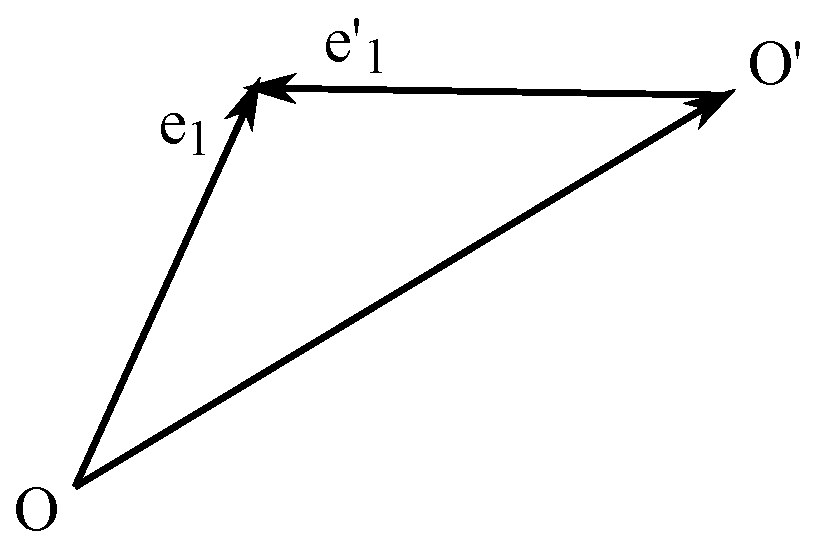
\includegraphics[width=0.5\columnwidth]{two-vectors-kiss}
    
      \caption{Концы соответственных базисных векторов, отложенных от соответствующих начал координат, совпадают.}
      \label{fig:two-vectors-kiss}
    \end{figure}
    
    Условие о том, что концы базисных векторов совпадают (при условии, что векторы отложены из начал систем координат), можно записать так (\ref{fig:two-vectors-kiss})
    \[
      \bds e_i = \vv{OO'} + \bds e_i'
    \]
    
    Нужно найти преобразование
    \[
      \bds x = S' \bds x' + \bds x(O')
    \]
    
    В то же время
    \[
      \bds e' = \bds e S'
    \]
    
    Поэтому матрицу $S'$ можно записать так
    \[
      S' = \begin{pmatrix}
        \begin{pmatrix}1\\ 0\\ 0\end{pmatrix} - \vv{OO'}_{\bds e}
        & \begin{pmatrix}0\\ 1\\ 0\end{pmatrix} - \vv{OO'}_{\bds e}
        & \begin{pmatrix}0\\ 0\\ 1\end{pmatrix} - \vv{OO'}_{\bds e}
      \end{pmatrix}
    \]
    где $\vv{OO'}_{\bds e}$~---~компоненты вектора $\vv{OO'}$ в базисе $\bds e$ (то же самое, что и $\bds x(O')$ в формуле, связывающей координаты точек).
    
    Получается, осталось лишь найти $\vv{OO'}$ в базисе $\bds e$.
    Это можно сделать, потому что мы учли ещё не всю информацию о взаимном расположении систем координат.
    На самом деле тот факт, что обе системы координат прямоугольные и концы соответственных векторов, отложенных из начал соответствующих систем координат, совпадают, означает, что у нас есть ``два поставленных друг на друга прямоугольных тетраэдра'' (\ref{fig:many-vectors-kisses}).
    
    \begin{figure}[h]
      \centering
    
      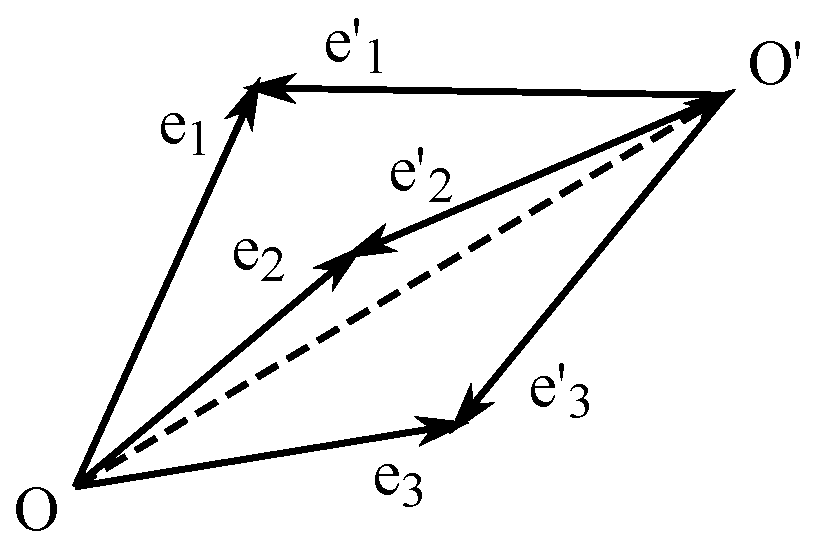
\includegraphics[width=0.5\columnwidth]{many-vectors-kisses}
    
      \caption{Базисы, отложенные от соответствующих начал координат~---~прямоугольные тетраэдры.}
      \label{fig:many-vectors-kisses}
    \end{figure}
    
    Поэтому вектор $\vv{OO'}$ можно найти как
    \[
      \vv{OO'} = 2 \cdot \left(\frac{1}{3} \bds e_1 + \frac{1}{3} \bds e_2 + \frac{1}{3} \bds e_3\right)
    \]
    (так как проекция точки пересечения $OO'$ с плоскостью концов базисных векторов на грани векторов $\bds e_i, \bds e_j$ совпадает с точкой пересечения медиан треугольников соответствующих граней\footnote{Точка $P$ пересечения $OO'$ с плоскостью концов базисных векторов $E_1 E_2 E_3$~---~очевидно, точка пересечения медиан $\triangle E_1 E_2 E_3$. То есть его центр масс. Если ``двигать'' одну из вершин $\triangle E_1 E_2 E_3$ по нормали до пересечения с гранью тетраэдра, скажем, двигать $E_3$ по нормали к плоскости $O E_1 E_2$, то она окажется вершиной $O$ при прямом угле в $\triangle O E_1 E_2$, а $P$ перейдёт в центр масс прямоугольного треугольника $O E_1 E_2$. Но положение проекции $P$ на грань $O E_1 E_2$ не менялось при сдвиге вершины $E_3$ по нормали к $O E_1 E_2$.}).
    
    Тогда матрица $S'$ равна
    \begin{equation}
    \begin{split}
      S' &= \begin{pmatrix}
        \begin{pmatrix}1\\ 0\\ 0\end{pmatrix} - \begin{pmatrix}2/3\\ 2/3\\ 2/3\end{pmatrix}
        & \begin{pmatrix}0\\ 1\\ 0\end{pmatrix} - \begin{pmatrix}2/3\\ 2/3\\ 2/3\end{pmatrix}
        & \begin{pmatrix}0\\ 0\\ 1\end{pmatrix} - \begin{pmatrix}2/3\\ 2/3\\ 2/3\end{pmatrix}
      \end{pmatrix}\\
      &= \begin{pmatrix}
        \begin{pmatrix}1/3\\ -2/3\\ -2/3\end{pmatrix}
        & \begin{pmatrix}-2/3\\ 1/3\\ -2/3\end{pmatrix}
        & \begin{pmatrix}-2/3\\ -2/3\\ 1/3\end{pmatrix}
      \end{pmatrix}\\
      &= \begin{pmatrix}
        1/3 & -2/3 & -2/3\\
        -2/3 & 1/3 & -2/3\\
        -2/3 & -2/3 & 1/3
      \end{pmatrix}
    \end{split}
    \end{equation}
  \end{solution}
\end{document}